\documentclass{proc}

\usepackage[backend=biber, style=trad-abbrv]{biblatex}
\usepackage{graphicx}
\usepackage{subfig}

\addbibresource{references.bib}

\title{Slipstream: Adaptive Co-Scheduling for Heterogenous Web Workloads}
\author{Fadhil Abubaker, Hussain Sadiq Abuwala}
\date{}

\begin{document}
\maketitle

\section{Motivation}

Present-day web applications process thousands of requests per second, each with
strict response times. Studies have shown that the average user will abandon a
web page if the load time is more than 3 seconds \cite{Akamai}. Hence, web
applications typically use background jobs to process long-running requests, as
well as any non-user-facing tasks. Executing background jobs involves a message
queue for queuing jobs, and a worker pool for processing them. Workers are
distributed across multiple nodes to support high-load scenarios. Figure 1 shows
an example of a web application that uses Celery \cite{Celery}, a popular
message queue for queuing jobs, with Celery workers running on multiple nodes.

An optimization metric in such a scenario is makespan, defined as the length of
time taken to complete a set of jobs. Increasing makespan typically equates to
spawning more workers, which in turn increases the number of jobs that can be
processed. However, care must be taken to spawn the right number of workers on
the given hardware. Eagerly spawning workers can lead to over-utilization of
hardware resources, which can worsen job completion times. On the other hand,
conservatively spawning workers can lead to under-utilization, leaving
performance improvements on the table.

\begin{figure}
  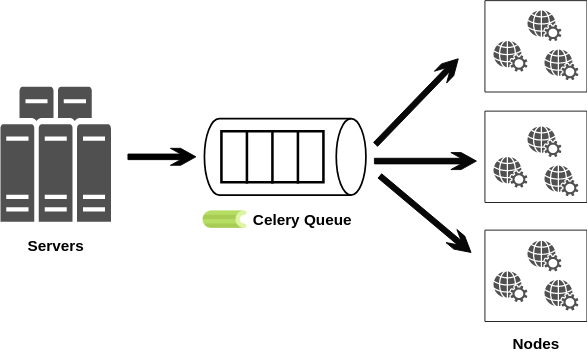
\includegraphics[width=\linewidth]{celery-diagram.png}
  \caption{A web application using Celery to queue jobs and execute them on workers.}
\end{figure}

The optimal number of workers to spawn is a function of workload
characteristics. If incoming jobs are CPU-bound, then the number of workers to
spawn per node is equal to the number of CPU cores on the node\footnote{This
assumes that jobs are single-threaded. This is a fair assumption, since most web
applications are written using frameworks in interpreted languages such as
Python and Ruby that use a global interpreter lock (GIL).}. If incoming jobs are
I/O-bound, then the number of workers to spawn per node is correlated with the
capacity of the I/O sub-system. Figure 2 shows makespan degradation on a node
with four cores as the number of jobs are increased, for both types of
workloads.

\begin{figure}
  \centering
  \subfloat[CPU-bound jobs]{{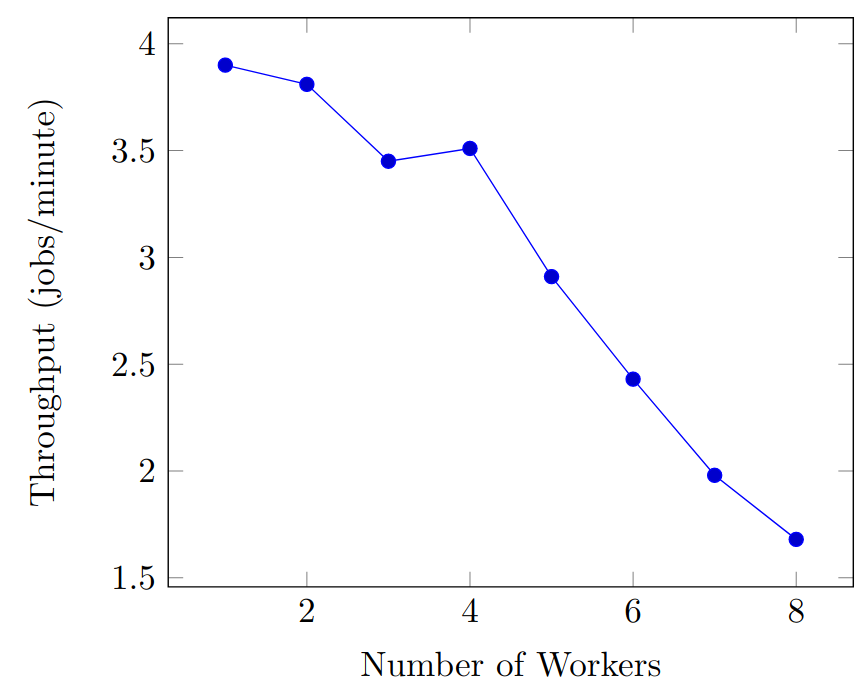
\includegraphics[width=5cm]{CPU-bound.png} }}%
  \qquad
  \subfloat[I/O-bound jobs]{{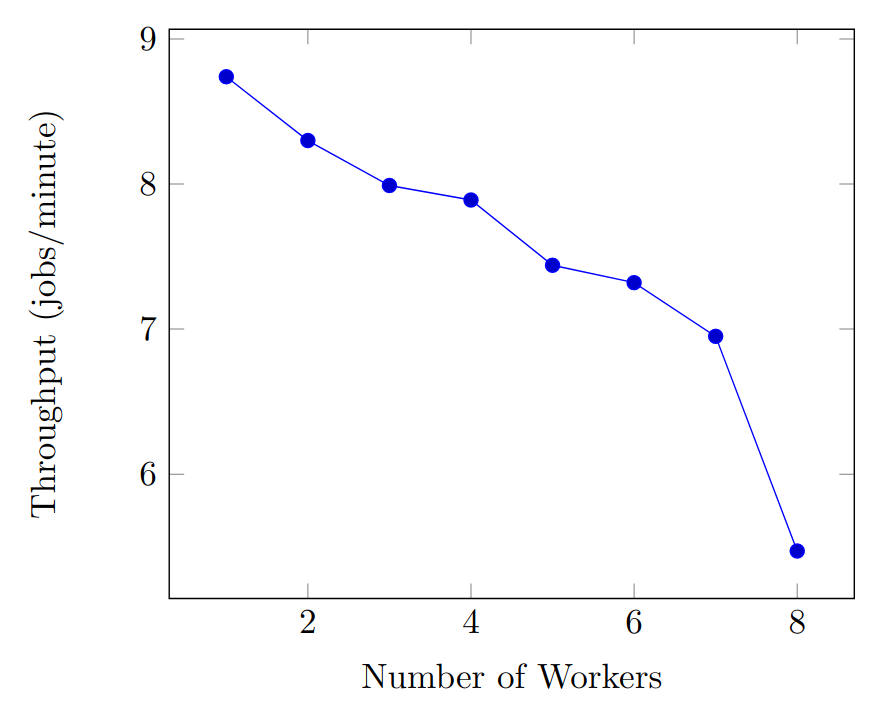
\includegraphics[width=5cm]{IO-bound.png} }}%
  \caption{Makespan degradation vs number of jobs on a node with four cores.}%
  \label{fig:example}%
\end{figure}

In practice, however, web workloads are heterogenous: they involve a mix of both
CPU and I/O-bound jobs. For example, an application could have jobs for training
models for learning user preferences (CPU-bound), as well as jobs that aggregate
data from multiple APIs (I/O-bound). One observation for maximizing makespan
of such workloads is that CPU-bound jobs can be co-scheduled with I/O-bound
jobs, since they use complementary resources \cite{10.1109/TPDS.2003.1206505}.

Using this observation, we build Slipstream, a scheduler for web workloads that
can adaptively co-schedule jobs to workers. Slipstream consists of two
components:
\begin{enumerate}
  \item An estimation model that can quantify the CPU and I/O characteristics of
  incoming jobs.
  \item A scheduling policy that uses the above estimation to spawn the optimal
  number of workers and assign jobs to them.
\end{enumerate}

Workload estimation in the data center setting has been studied in the past
\cite{186175, 8478443, 5279616}. Additionally, the idea of co-scheduling
CPU-bound and I/O-bound processes on large clusters has also been explored
\cite{5279616, 10.1109/TPDS.2003.1206505}. Slipstream is partly inspired by
these techniques, and looks at how they can be adapted to execution backends
used by small to mid-sized web applications.

\section{Methodology}

We will build Slipstream on top of RQ \cite{RQ}, a Python library that uses Redis
for queueing jobs and executing them on workers. Slipstream will run as an
independent service that monitors the job queue, spawns workers, assigns jobs
and profiles job execution to learn the characteristics of its workload. At
first, a conservative number of workers will be spawned. Gradually, as the
system learns the workload characteristics of each job, more workers will be
spawned and jobs will be assigned to them using a workload-aware scheduling
policy.

To evaluate Slipstream, we will use jobs with varying inputs that emulate the
mixed workloads seen in a typical web application such as machine-learning and
data-gathering jobs. We then compare it against static scheduling policies that
allocate a fixed number of workers to each node. The expectation is that
Slipstream will exhibit better makespan due to more effective utilization of
resources.

\printbibliography
\end{document}
